%! Author = nadutkinfedor
%! Date = 16.01.2024

% Preamble
\documentclass[11pt]{article}
\usepackage[left=2cm, right=1cm, top=2cm, bottom=2cm, bindingoffset=0cm]{geometry}

% Packages
\usepackage[utf8]{inputenc}
\usepackage[russian]{babel}
\usepackage{amsmath}
\usepackage{hyperref}
\usepackage{graphicx}
\usepackage{misccorr}
\usepackage{listings}
\usepackage{xcolor}
\usepackage{titlesec}
\usepackage{minted}
\usepackage{color}
\usepackage{enumitem}
\usepackage{indentfirst}

%listing settings
\definecolor{dkgreen}{rgb}{0,0.6,0}
\definecolor{gray}{rgb}{0.5,0.5,0.5}
\definecolor{mauve}{rgb}{0.58,0,0.82}

\lstset{ %
    backgroundcolor=\color{white},   % choose the background color
    basicstyle=\footnotesize,        % size of fonts used for the code
    breaklines=true,                 % automatic line breaking only at whitespace
    captionpos=b,                    % sets the caption-position to bottom
    commentstyle=\color{dkgreen},    % comment style
    escapeinside={\%*}{*},          % if you want to add LaTeX within your code
    keywordstyle=\color{blue},       % keyword style
    stringstyle=\color{mauve},     % string literal style
}

% Title
\title{Параллельные алгоритмы}
\author{Надуткин Федор }
\date{January 2023}

\titleformat{\section}[block]{\Huge\bfseries\filcenter}{}{1em}{}
\titleformat{\subsection}[block]{\huge\bfseries\filcenter}{}{1em}{}
\titleformat{\subsubsection}[block]{\Large\bfseries\filcenter}{}{1em}{}

% Document
\begin{document}

    \maketitle
    \newpage

    \section*{Pipelining}

    Идея \texttt{pipelining} - идея конвейера, делать всё поэтапно и для новой детали начинать выполнение первого этапа,
    пока старая деталь уже на втором.

    \subsection*{Задача: Вставить в \texttt{2-3} дерево $m$ элементов.}

    \begin{figure}[h!]
        \centering
        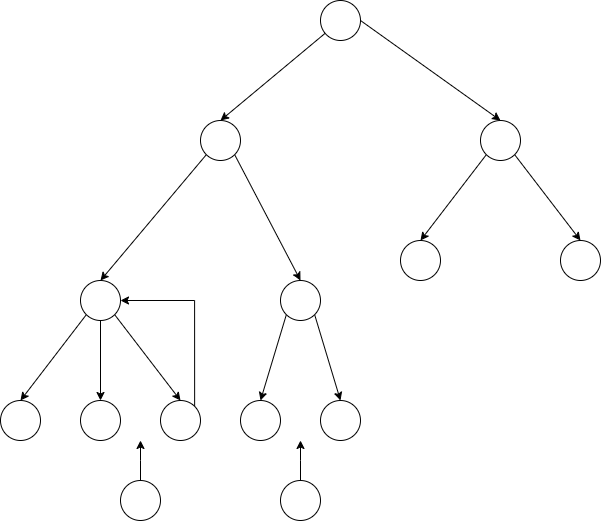
\includegraphics[width=0.7\textwidth]{Pictures/Pipelining/2-3}
        \caption{Вставка в 2--3 дерево}
        \label{fig:2-3_tree}
    \end{figure}

    \begin{enumerate}
        \item Находим куда надо вставить элемент.
        \item Вставляем, если у вершины 2 ребёнка, то останавливаемся, если 3, то делаем сплит и поднимаемся выше.
        \item Если 2 или 3 потока пришли делать split, то выбираем главного и он уже идёт делить дальше.
    \end{enumerate}

    \texttt{Work} = $m \cdot \log{(n + m)}$

    \texttt{Span} = $\log{m} + \log{n}$
    
    \subsubsection*{Проблема:}

    Если у нас на первом этапе вставляется множество элементов в одно место, то делать split не получится.


    \subsubsection*{Решение:}

    \begin{enumerate}
        \item Взять центральный элемент из массива тех, что нам надо вставить.
        \item Вставить этот элемент в \texttt{2-3 дерево}.
        \item Делать процедуру уже для 2 массивов, между которыми уже будет ключ.
    \end{enumerate}

    \texttt{Span} = $\log{1} \cdot \log{n} + \log{2} \cdot \log{n} + \dots + \log{m} \cdot \log{n} = \mathcal{O}(\log^2{m} \cdot \log{n})$
    
    \subsubsection*{Ускорение:}

    Стоит заметить, что нам не нужно доводить элементы до самого верха, чтобы вставить новые.
    По прошествии 2 итераций новые элементы никак не будут взаимодействовать со старыми, а значит не помешают.
    Поэтому алгоритм изменится следующим образом:

    \begin{enumerate}
        \item Взять центральный элемент.
        \item Вставить элемент в \texttt{2-3 дерево}.
        \item Проделать 2 итерации для всех незавершённых элементов.
        \item Сделать процедуру для 2 массивов.
    \end{enumerate}

    \texttt{Span} = $\log{m} \cdot (\log{n} + \log{m}) = \log{m} \cdot \log{n} + \log^2{m}$

    \section*{Symmetry breaking}

    \begin{figure}[h!]
        \centering
        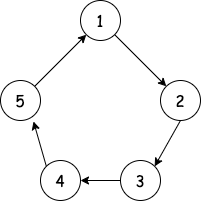
\includegraphics[width=0.4\textwidth]{Pictures/Symmetry breaking/Symmetry breaking}
        \caption{Symmetry breaking}
        \label{fig:symmetry_breaking}
    \end{figure}

    Для каждой вершины дано \texttt{next[id]}, нужно найти \texttt{prev[id]}.
    Делаем \texttt{parallel for} и устанавливаем \texttt{prev[next[id]] = id}.

    \subsection*{Задача}
    Раскрасить в минимальное число цветов граф.

    \subsection*{Решение}

    \begin{figure}[h!]
        \centering
        
\includegraphics[width=0.4\textwidth]{Pictures/Symmetry breaking/Symmetry breaking proof}
        \caption{Берём x и next[x]}\label
        {fig:symmetry_breaking_proof}
    \end{figure}

    Переведём $x$ и $y$ в двоичную форму.
    $x$ = \texttt{001101}, $y$ = \texttt{000101}.
    \texttt{color[y]} = $2 \cdot \min{(bit_{color[x] \neq color[y]})} + bit_{color[y]} = 2 \cdot 3 + 0$.
    Изначально \texttt{color} каждой вершины равен её id.

    Стоит заметить, что $\forall$ двух соседних вершин, их цвета не равны.
    Если \texttt{color[id]} с \texttt{color[id + 1]} и \texttt{color[id + 1]} с \texttt{color[id + 2]} различаются в разных битах (например \texttt{color[id]} с \texttt{color[id + 1]} меньше), то и разница между ними будет как минимум 2.
    Если же они различаются в одной и той же позиции, то тогда \texttt{color[id + 1]} и \texttt{color[id + 2]} имеют разный бит на этой позиции.

    Каждый раз количество цветов уменьшается в $\log$ раз, поэтому можно дойти до момента $n \rightarrow 2 \cdot \log{n} \rightarrow 2 \cdot \log{(\log{n})} \rightarrow \dots C$, где $C$ - некоторая константа.
    Однако $C$ может оказаться больше, чем $3$.
    Для решения этой проблемы, для каждого цвета составим массив из вершин этого цвета.

    \begin{figure}[h!]
        \centering
        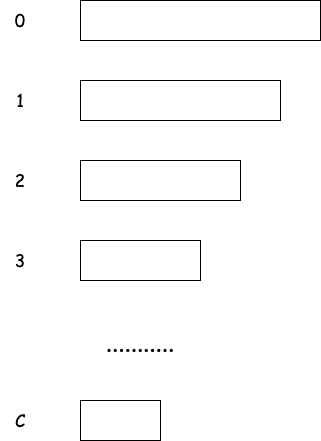
\includegraphics[width=0.4\textwidth]{Pictures/Symmetry breaking/Diagram Painting}
        \caption{Массивы с вершинами.}
        \label{fig:painting}
    \end{figure}

    \begin{enumerate}
        \item Вставляем все вершины из \texttt{0}, \texttt{1}, \texttt{2} (не получатся одинаковыми по прошлому рассуждению).
        \item Для всех последующих списков, берём вершину из списка и красим её в минимальный цвет (0, 1, 2), которого не было у соседей, так как соседей 2, а цветов 3 это возможно (если соседи не покрашены, то делаем $\min$ с цветами, которые есть).
    \end{enumerate}

    \texttt{Work} = $n \cdot \log^2{n}$

    \texttt{Span} = $polylog(n)$

    \section*{List Ranking}

    У нас есть одно связанный список, для каждой вершины известно \texttt{next[id]}, надо найти расстояние от каждой вершины до конца.

    \begin{figure}[h!]
        \centering
        
\includegraphics[width=0.4\textwidth]{Pictures/List Ranking/List Ranking}
        \caption{Односвязанный список}
        \label{fig:list_ranking}
    \end{figure}
    
    \subsection*{Решения}
    
    \subsubsection*{Двоичные подъёмы}

    \begin{figure}[h!]
        \centering
        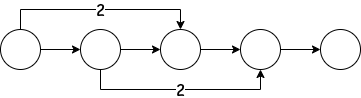
\includegraphics[width=0.4\textwidth]{Pictures/List Ranking/Binary lifts}
        \caption{Двоичные подъёмы.}
        \label{fig:binary_lifts}
    \end{figure}
    
    \begin{lstlisting}[label={lst:binary_lifts}]
        pfor i=1...n
            next'[i] = next[i] + next[next[i]]
            len'[i] = len[i] + len[next[i]]
    \end{lstlisting}

    \texttt{Work} = $n \cdot \log{n}$

    \texttt{Span} = $\log^2{n}$

    \subsubsection*{Уменьшение работы при помощи Symmetry breaking}

    \begin{enumerate}
        \item При помощи \texttt{Symmetry breaking} раскрашиваем вершины в 3 цвета.
        \begin{figure}[h!]
            \centering
            
\includegraphics[width=0.4\textwidth]{Pictures/List Ranking/Symmetry breaking list ranking}
            \label{fig:symmetry_breaking_list_ranking}
        \end{figure}
        \item Удаляем вершины с номером 2.
        \begin{figure}[h!]
            \centering
            
\includegraphics[width=0.4\textwidth]{Pictures/List Ranking/Deleting nodes}
            \label{fig:deleting_nodes_list_ranking}
        \end{figure}
        \item Когда количество вершин станет равным $\frac{n}{\log{n}}$ запускаем алгоритм \texttt{List Ranking}.
        \item После этого начинаем возвращать вершины, мы знаем, что у вершины цвета 2 нет соседа цвета 2 $\Rightarrow$ мы знаем расстояние от её соседа до конца, а значит \texttt{len[id] = len[next[id]] + 1}.
    \end{enumerate}

    \texttt{Work} $= \mathcal{O}(n)$

    \texttt{Span} = $= \mathcal{O}(\log^2{n} \cdot \log{\log{n}})$

    \subsubsection*{Randomized List Ranking}

    Метод позволяющий сократить количество вершин перед \texttt{List Ranking}.

    \begin{enumerate}
        \item Для каждой вершины подбрасываем монетку \texttt{Head} или \texttt{Tail}.
        \begin{figure}[h!]
            \centering
            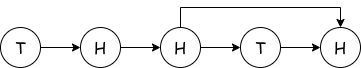
\includegraphics[width=0.4\textwidth]{Pictures/List Ranking/Randomized List Ranking}
            \label{fig:head_tail}
        \end{figure}
        \item Удалим все вершины \texttt{H} у которых \texttt{next} это \texttt{T}.
        Ожидаемое количество удалённых вершин $= \frac{n}{4}$.
        Попытка удачная, если нам удалось удалить $\frac{7}{8}$ вершин.
        \item Дальше всё так же как и в \texttt{List Ranking с Symmetry Breaking}.
    \end{enumerate}
\end{document}